
\paragraph{UC-30 Completamento della registrazione da parte del nuovo utente}

	\begin{itemize}
		\item \textbf{Attore primario:} utente non registrato;

		\item \textbf{Descrizione:} l'utente vuole completare la registrazione presso il sistema inserendo i propri dati anagrafici e la propria password personale. Tutti i campi dati richiesti sono obbligatori;

		\item \textbf{Precondizioni:} l'utente ha cliccato il link per completare la registrazione ricevuto via mail;

		\item \textbf{Postcondizioni:} l'utente è registrato presso il sistema;

		\item \textbf{Scenario principale:}
	      \begin{enumerate}
		      \item l'utente inserisce il proprio nome nell'apposito form (UC-30.1 Inserimento nome);
		      \item l'utente inserisce il proprio cognome nell'apposito form (UC-30.2 Inserimento cognome);
		      \item l'utente inserisce la propria password personale nell'apposito form (UC-30.3 Inserimento password);
		      \item l'utente inserisce nuovamente la password per confermarla (UC-30.4 Conferma password);
		      \item l'utente invia i dati al sistema il quale elabora la richiesta e completa la registrazione del nuovo utente;
	      \end{enumerate}
	\end{itemize}

	\begin{figure}[H]
		\centering
		  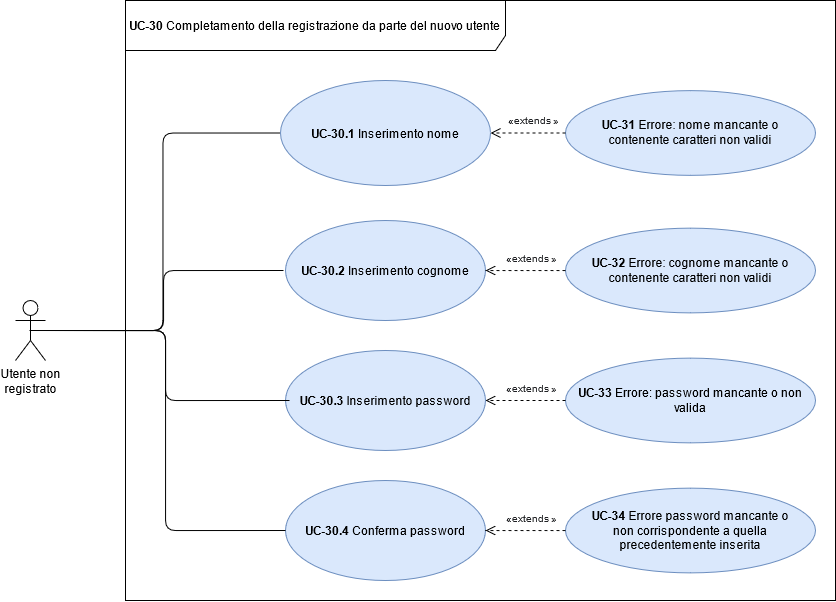
\includegraphics[scale=0.45]{src/CasiDUso/immagini/CompletamentoRegistrazione.png}
		\caption{Diagramma relativo alal completamento della registrazione da parte dell'utente}
	\end{figure}
	


\paragraph{UC-30.1 Inserimento nome}

	\begin{itemize}
		\item \textbf{Attore primario:} utente non registrato;

		\item \textbf{Descrizione:} l'utente vuole inserire il proprio nome per registrarsi presso il sistema. Il nome non può contenere caratteri speciali o numeri;

		\item \textbf{Precondizioni:} l'utente ha selezionato il form preposto all'inserimento del proprio nome;

		\item \textbf{Postcondizioni:} l'utente ha inserito con successo il proprio nome;

		\item \textbf{Scenario principale:}
	  	  \begin{enumerate}
		  	\item l'utente digita il proprio nome all'interno dell'apposito form;
	      \end{enumerate}
		\item \textbf{Estensioni:}
	      \begin{itemize}
		      \item UC-31 Errore: nome mancante o contenente caratteri non validi.
	      \end{itemize}
	\end{itemize}

\paragraph{UC-30.2 Inserimento cognome}

	\begin{itemize}
		\item \textbf{Attore primario:} utente non registrato;

		\item \textbf{Descrizione:} l'utente vuole inserire il proprio cognome per registrarsi presso il sistema. Il cognome non può contenere caratteri speciali o numeri;

		\item \textbf{Precondizioni:} l'utente ha selezionato il form preposto all'inserimento del proprio cognome;

		\item \textbf{Postcondizioni:} l'utente ha inserito con successo il proprio cognome;

		\item \textbf{Scenario principale:}
			\begin{enumerate}
		  		\item l'utente digita il proprio cognome all'interno dell'apposito form;
	  		\end{enumerate}
		\item \textbf{Estensioni:}
	  		\begin{itemize}
		  		\item UC-32 Errore: cognome mancante o contenente caratteri non validi.
	  		\end{itemize}
	\end{itemize}

\paragraph{UC-30.3 Inserimento password}

	\begin{itemize}
		\item \textbf{Attore primario:} utente non registrato;

		\item \textbf{Descrizione:} l'utente inserire vuole inserire la propria password personale per registrarsi presso il sistema. Il cognome non può contenere caratteri speciali (es.spazi);

		\item \textbf{Precondizioni:} l'utente ha selezionato il form preposto all'inserimento della nuova password;

		\item \textbf{Postcondizioni:} l'utente ha inserito con successo la propria password;

		\item \textbf{Scenario principale:}
			\begin{enumerate}
		  		\item l'utente digita la nuova password all'interno dell'apposito form;
	  		\end{enumerate}
		\item \textbf{Estensioni:}
	  		\begin{itemize}
		  		\item UC-33 Errore: password mancante o non valida.
	  		\end{itemize}
	\end{itemize}

\paragraph{UC-30.4 Conferma password}

	\begin{itemize}
		\item \textbf{Attore primario:} utente non registrato;
	
		\item \textbf{Descrizione:} l'utente inserire confermare la propria password per registrarsi presso il sistema. \`{E} richiesto pertanto di inserire nuovamente la password in un apposito form;

		\item \textbf{Precondizioni:} l'utente ha selezionato il form preposto alla conferma della nuova password;

		\item \textbf{Postcondizioni:} l'utente ha confermato con successo la propria password;

		\item \textbf{Scenario principale:}
			\begin{enumerate}
		  		\item l'utente conferma la propria password inserendola nell'apposito form;
	  		\end{enumerate}
		\item \textbf{Estensioni:}
	  		\begin{itemize}
		  		\item UC-34 Errore: password mancante o non corrispondente a quella precedentemente inserita.
	  		\end{itemize}
	\end{itemize}

\paragraph{UC-31 Errore: nome mancante o contenente caratteri non validi}

	\begin{itemize}
		\item \textbf{Attore primario:} utente non registrato;

		\item \textbf{Descrizione:} l'utente non ha inserito il proprio cognome o ha digitato caratteri non validi (numeri,spazi, segni di punteggiatura) nel form dedicato all'inserimento del proprio nome. Viene visualizzato un messaggio d'errore esplicativo e la registrazione non viene completata;

		\item \textbf{Precondizioni:} l'utente non ha inserito il proprio cognome o ha inserito dei caratteri non validi e ha inviato i dati al sistema;

		\item \textbf{Postcondizioni:} il sistema restituisce un messaggio d'errore esplicativo e non completa la fase di registrazione dell'utente;

		\item \textbf{Scenario principale:}
	  		\begin{enumerate}
		  		\item il sistema elabora la richiesta ricevuta e mostra a video un messaggio d'errore esplicativo senza completare la richiesta di registrazione dell'utente; 
	  		\end{enumerate}
	\end{itemize}
 

\paragraph{UC-32 Errore: cognome mancante o contenente caratteri non validi}

	\begin{itemize}
		\item \textbf{Attore primario:} utente non registrato;

		\item \textbf{Descrizione:} l'utente ha inserito una coppia di credenziali non riconosciuta dal sistema e ha inviato i propri dati;

		\item \textbf{Precondizioni:} l'utente ha inserito il proprio indirizzo email e la propria password;

		\item \textbf{Postcondizioni:} il sistema restituisce un messaggio d'errore esplicativo e non completa la fase di registrazione dell'utente;

		\item \textbf{Scenario principale:}
	  		\begin{enumerate}
		  		\item il sistema elabora la richiesta ricevuta e mostra a video un messaggio d'errore esplicativo senza completare la richiesta di registrazione dell'utente; 
	  		\end{enumerate}
	\end{itemize}

\paragraph{UC-33 Errore: password mancante o non valida}

	\begin{itemize}
		\item \textbf{Attore primario:} utente non registrato;

		\item \textbf{Descrizione:} l'utente non ha inserito la password o ha inserito caratteri speciali o non rispetta i vincoli di lunghezza all'interno del form preposto all'inserimento di una nuova password e ha inviato i propri dati;

		\item \textbf{Precondizioni:} l'utente non ha inserito la password o ha inserito caratteri speciali o non rispetta i vincoli di lunghezza all'interno del form preposto all'inserimento di una nuova password e ha inviato i propri dati;

		\item \textbf{Postcondizioni:} il sistema restituisce un messaggio d'errore esplicativo e non completa la fase di registrazione dell'utente;

		\item \textbf{Scenario principale:}
	  		\begin{enumerate}
		  		\item il sistema elabora la richiesta ricevuta e mostra a video un messaggio d'errore esplicativo senza completare la richiesta di registrazione dell'utente; 
	  		\end{enumerate}
	\end{itemize}


\paragraph{UC-34 Errore: password mancante o non corrispondente a quella precedentemente inserita}

	\begin{itemize}
		\item \textbf{Attore primario:} utente non registrato;

		\item \textbf{Descrizione:} viene visualizzato un messaggio d'errore poiché l'utente non ha confermato correttamente la propria password;

		\item \textbf{Precondizioni:} l'utente ha inserito una password diversa da quella precedentemente inserita e ha inviato i dati al sistema;

		\item \textbf{Postcondizioni:} il sistema restituisce un messaggio d'errore esplicativo e non completa la fase di registrazione dell'utente;

		\item \textbf{Scenario principale:}
	  		\begin{enumerate}
		  		\item il sistema elabora la richiesta ricevuta e mostra a video un messaggio d'errore esplicativo senza completare la richiesta di registrazione dell'utente; 
	  		\end{enumerate}
	\end{itemize}

\paragraph{UC-35 Login mobile}

	\begin{itemize}
		\item \textbf{Attore primario:} utente non autenticato;

		\item \textbf{Descrizione:} l'utente vuole autenticarsi presso il sistema inserendo le proprie credenziali (indirizzo e-mail e password). L'autenticazione non va a buon fine qualora la coppia di credenziali non sia riconosciuta dal sistema;

		\item \textbf{Precondizioni:} l'utente ha avviato l'applicazione mobile;

		\item \textbf{Postcondizioni:} l'utente è autenticato presso il sistema e può visualizzare la propria dashboard personale;

		\item \textbf{Scenario principale:}
	  		\begin{enumerate}
		  		\item l'utente seleziona la funzionalità di login;
		  		\item l'utente inserisce le proprie credenziali all'interno del form per l'autenticazione (UC-35.1 Inserimento delle credenziali per il login);
		  		\item l'utente invia i dati al sistema;
		  		\item il sistema completa la richiesta di autenticazione qualora le credenziali vengano riconosciute e aggiorna la schermata del dispositivo con la dashboard personale dell'utente. In caso contrario l'autenticazione non viene completata e si rimane nella pagina di login.
	  		\end{enumerate}
	\end{itemize}

	\begin{figure}[H]
		\centering
		  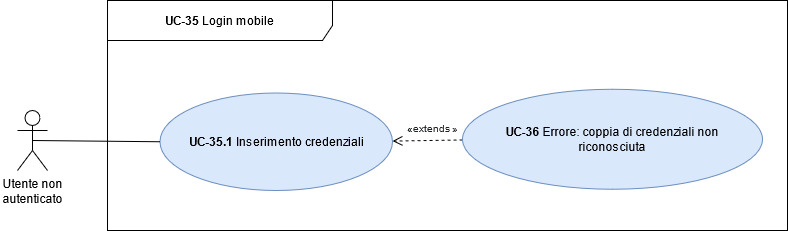
\includegraphics[scale=0.50]{src/CasiDUso/immagini/LoginMobile.png}
		\caption{Diagramma relativo all'autenticazione presso l'applicazione mobile}
	\end{figure}

\paragraph{UC-35.1 Inserimento delle credenziali per il login}

	\begin{itemize}
		\item \textbf{Attore primario:} utente non autenticato;

		\item \textbf{Descrizione:} l'utente vuole inserire le proprie credenziali nell'apposito form nella schermata di login;

		\item \textbf{Precondizioni:} l'utente ha selezionato selezionato la funzionalità di login;

		\item \textbf{Postcondizioni:} l'utente ha inserito con successo le proprie credenziali;

		\item \textbf{Scenario principale:}
	  		\begin{enumerate}
		  		\item l'utente inserisce il proprio indirizzo email nell'apposito form nella schermata di login (UC-35.1.1 Inserimento dell'indirizzo email per il login); 
		  		\item l'utente inserisce la propria password nell'apposito form nella schermata di login (UC-35.1.2 Inserimento della password per il login).
	  		\end{enumerate}
	    \item \textbf{Estensioni:}
	  		\begin{itemize}
		  		\item UC-36 Errore: coppia di credenziali non riconosciuta dal sistema.
	  		\end{itemize}
	\end{itemize}

	\begin{figure}[H]
		\centering
		  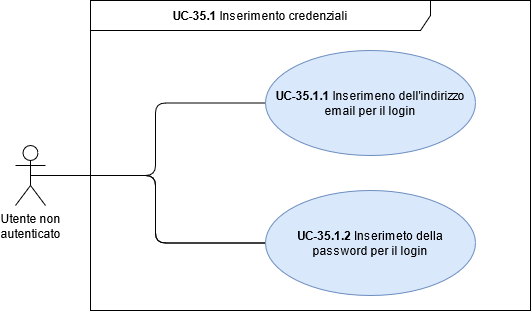
\includegraphics[scale=0.50]{src/CasiDUso/immagini/InserimentocredenzialiMobile.png}
		\caption{Diagramma relativo all'inserimento delle credenziai per il login da applicazione mobile}
	\end{figure}


\paragraph{UC-35.1.1 Inserimento dell'indirizzo email per il login}

	\begin{itemize}
		\item \textbf{Attore primario:} utente non autenticato;

		\item \textbf{Descrizione:} l'utente vuole inserire il proprio indirizzo email nell'apposito form nella schermata di login;

		\item \textbf{Precondizioni:} l'utente ha selezionato il form per l'inserimento dell'indirizzo email;

		\item \textbf{Postcondizioni:} l'utente ha inserito con successo il proprio indirizzo email;

		\item \textbf{Scenario principale:}
	  		\begin{enumerate}
		  		\item l'utente inserisce il proprio indirizzo email nell'apposito form nella schermata di login; 
	  		\end{enumerate}
	\end{itemize}

\paragraph{UC-35.1.2 Inserimento della password per il login}

	\begin{itemize}
		\item \textbf{Attore primario:} utente non autenticato;

		\item \textbf{Descrizione:} l'utente vuole inserire la propria password nell'apposito form nella schermata di login;

		\item \textbf{Precondizioni:} l'utente ha selezionato il form per l'inserimento della password;

		\item \textbf{Postcondizioni:} l'utente ha inserito con successo la propria password;

		\item \textbf{Scenario principale:}
	  		\begin{enumerate}
			  \item l'utente inserisce la propria password nell'apposito form nella schermata di login; 
	  		\end{enumerate}
	\end{itemize}

\paragraph{UC-36 Errore: coppia di credenziali non riconosciuta dal sistema}

	\begin{itemize}
		\item \textbf{Attore primario:} utente non autenticato;

		\item \textbf{Descrizione:} l'utente ha inserito una coppia di credenziali non riconosciuta dal sistema e ha inviato i propri dati;

		\item \textbf{Precondizioni:} l'utente ha inserito il proprio indirizzo email e la propria password;

		\item \textbf{Postcondizioni:} il sistema restituisce un messaggio d'errore esplicativo e non completa la fase di autenticazione dell'utente;

		\item \textbf{Scenario principale:}
	  		\begin{enumerate}
		  		\item il sistema elabora la richiesta ricevuta e mostra a video un messaggio d'errore esplicativo senza completare la richiesta di autenticazione; 
	  		\end{enumerate}
	\end{itemize}

\paragraph{UC-37 Recupero password da applicazione mobile}

	\begin{itemize}
		\item \textbf{Attore primario:} utente non autenticato;

		\item \textbf{Descrizione:} l'utente vuole poter modificare la propria password dalla schermata di login tramite un link per il recupero della password ;

		\item \textbf{Precondizioni:} l'utente ha avviato l'applicazione mobile e non si ricorda la propria password;

		\item \textbf{Postcondizioni:} l'utente ha modificato con successo la propria password;

		\item \textbf{Scenario principale:}
	  		\begin{enumerate}
		  		\item l'utente clicca il link per il recupero password; 
		  		\item l'utente inserisce l'indirizzo email al quale inviare il link per il reset della password (UC-37.1 Inserimento mail di registrazione);
		  		\item l'utente inserisce la nuova password (UC-37.2 inserimento nuova password);
		  		\item l'utente conferma la nuova password (UC-37.3 conferma nuova password);
		  		\item l'utente invia i dati al sistema.
		  		\item il sistema modifica la password dell'utente qualora la procedura sia stata eseguita in modo corretto.
	  		\end{enumerate}
	\end{itemize}

	\begin{figure}[H]
		\centering
		  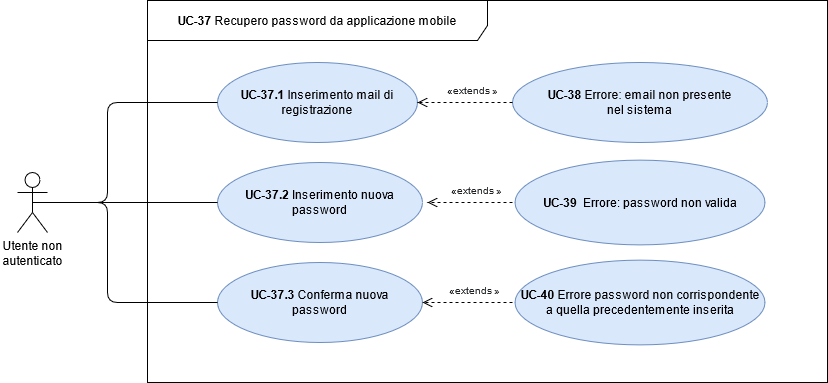
\includegraphics[scale=0.50]{src/CasiDUso/immagini/RecuperoPasswordMobile.png}
		\caption{Diagramma relativo al recupero password da applicazione mobile}
	\end{figure}

\paragraph{UC-37.1 Inserimento mail di registrazione}

	\begin{itemize}
		\item \textbf{Attore primario:} utente non autenticato;

		\item \textbf{Descrizione:} l'utente vuole inserire la propria mail di registrazione per ricevere il link di modifica della password;

		\item \textbf{Precondizioni:} l'utente ha selezionato il form di inserimento dell'indirizzo email nella procedura di recupero password;

		\item \textbf{Postcondizioni:} l'utente ha inserito con successo l'indirizzo email per la ricezione del link di modifica della password;

		\item \textbf{Scenario principale:}
	  		\begin{enumerate}
		  		\item l'utente inserisce la mail con la quale è registrato presso ; 
	  		\end{enumerate}
	  	\item \textbf{Estensioni:}
	  		\begin{itemize}
		  		\item UC-38 Errore: indirizzo email mancante o non presente nel sistema.
	  		\end{itemize}
		\end{itemize}

\paragraph{UC-37.2 Inserimento nuova password}

	\begin{itemize}
		\item \textbf{Attore primario:} utente non autenticato;

		\item \textbf{Descrizione:} l'utente vuole inserire la nuova password con la quale autenticarsi;

		\item \textbf{Precondizioni:} l'utente ha cliccato il link per il reset della password ricevuto via mail;

		\item \textbf{Postcondizioni:} l'utente ha inserito con successo la nuova password;

		\item \textbf{Scenario principale:}
	  		\begin{enumerate}
		  		\item l'utente seleziona il form per l'inserimento della nuova password;
		  		\item l'utente inserisce la nuova password.
	  		\end{enumerate}
	  	\item \textbf{Estensioni:}
	  		\begin{itemize}
		  		\item UC-39 Errore: password mancante o non valida.
	  		\end{itemize}
	\end{itemize}

\paragraph{UC-37.3 Conferma nuova password}

	\begin{itemize}
		\item \textbf{Attore primario:} utente non autenticato;

		\item \textbf{Descrizione:} all'utente è richiesto di confermare la password inserita. \`{E} necessario il reinserimento della password in un apposito form;

		\item \textbf{Precondizioni:} l'utente ha inserito la nuova password;

		\item \textbf{Postcondizioni:} l'utente ha confermato con successo la nuova password;

		\item \textbf{Scenario principale:}
	  		\begin{enumerate}
		  		\item l'utente seleziona il form per la conferma della nuova password;
		  		\item l'utente inserisce la stessa password precedentemente inserita.
		  		\item il sistema confronta le due password. Se esse coincidono viene completata correttamente la procedura di recupero password.
	  		\end{enumerate}
	  	\item \textbf{Estensioni:}
	  		\begin{itemize}
		  		\item UC-40 Errore: password non corrispondente a quella precedentemente inserita.
	  		\end{itemize}
	\end{itemize}

\paragraph{UC-38 Errore: mail mancante o non presente nel sistema}

	\begin{itemize}
		\item \textbf{Attore primario:} utente non autenticato;

		\item \textbf{Descrizione:} l'utente non ha inserito;

		\item \textbf{Precondizioni:} l'utente non ha inserito il proprio cognome o ha inserito dei caratteri non validi e ha inviato i dati al sistema;

		\item \textbf{Postcondizioni:} il sistema restituisce un messaggio d'errore esplicativo e non completa la fase di recupero password;

		\item \textbf{Scenario principale:}
	  		\begin{enumerate}
		  		\item il sistema elabora la richiesta ricevuta e mostra a video un messaggio d'errore esplicativo senza completare la richiesta di recupero password; 
	  		\end{enumerate}
	\end{itemize}

\paragraph{UC-39 Errore: password mancante o non valida}

	\begin{itemize}
		\item \textbf{Attore primario:} utente non autenticato;

		\item \textbf{Descrizione:} viene visualizzato un messaggio d'errore esplicativo poiché l'utente non ha inserito la password o la password inserita non rispetta i vincoli di lunghezza o contiene caratteri speciali;

		\item \textbf{Precondizioni:} l'utente non ha inserito la propria password o ha inserito una password non valida e ha inviato i dati al sistema;

		\item \textbf{Postcondizioni:} il sistema restituisce un messaggio d'errore esplicativo e non completa la fase di recupero password;

		\item \textbf{Scenario principale:}
	  		\begin{enumerate}
		  		\item il sistema elabora la richiesta ricevuta e mostra a video un messaggio d'errore esplicativo senza completare la richiesta di recupero password; 
	  		\end{enumerate}
	\end{itemize}

\paragraph{UC-40 Errore: password non corrispondente a quella precedentemente inserita}

	\begin{itemize}
		\item \textbf{Attore primario:} utente non autenticato;

		\item \textbf{Descrizione:}  viene visualizzato un messaggio d'errore poiché l'utente non ha confermato correttamente la propria password;

		\item \textbf{Precondizioni:} l'utente ha inserito una password diversa da quella precedentemente digitata e ha inviato i dati al sistema;

		\item \textbf{Postcondizioni:} il sistema restituisce un messaggio d'errore esplicativo e non completa la fase di recupero password;

		\item \textbf{Scenario principale:}
	  		\begin{enumerate}
		  		\item il sistema elabora la richiesta ricevuta e mostra a video un messaggio d'errore esplicativo senza completare la richiesta di recupero password; 
	  		\end{enumerate}
	\end{itemize}

\paragraph{UC-41 Modifica password da applicazione mobile}

	\begin{itemize}
		\item \textbf{Attore primario:} utente autenticato;

		\item \textbf{Descrizione:}  l'utente vuole poter modificare la propria password dalla propria area personale;

		\item \textbf{Precondizioni:} l'utente ha selezionato la funzionalità di modifica della password dalla propria area personale;

		\item \textbf{Postcondizioni:} l'utente ha modificato con successo la propria password;

		\item \textbf{Scenario principale:}
	  		\begin{enumerate}
		  		\item l'utente inserisce la password corrente (UC-41.1 Inserimento password corrente);
		  		\item l'utente inserisce la nuova password (UC-41.2 Inserimento nuova password);
		  		\item l'utente conferma la nuova password (UC-41.3 Conferma nuova password);
		  		\item l'utente invia i dati al sistema;
		  		\item il sistema modifica la password dell'utente qualora la procedura sia stata eseguita in modo corretto.
	  		\end{enumerate}
	\end{itemize}

	\begin{figure}[H]
		\centering
		  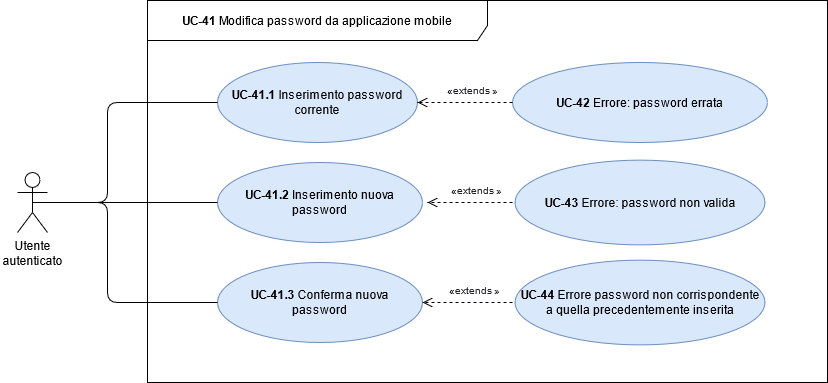
\includegraphics[scale=0.50]{src/CasiDUso/immagini/ModificaPasswordMobile.png}
		\caption{Diagramma relativo alla modifica della password da applicazione mobile}
	\end{figure}

\paragraph{UC-41.1 Inserimento password corrente}

	\begin{itemize}
		\item \textbf{Attore primario:} utente autenticato;

		\item \textbf{Descrizione:} l'utente vuole inserire la password corrente per confermare la propria identità;

		\item \textbf{Precondizioni:} l'utente ha selezionato il form di inserimento della password corrente;

		\item \textbf{Postcondizioni:} l'utente ha inserito con successo la password corrente;

		\item \textbf{Scenario principale:}
	  		\begin{enumerate}
		  		\item l'utente digita la password corrente nel form selezionato.
	  		\end{enumerate}
		\item \textbf{Estensioni:}
			\begin{itemize}
		  		\item UC-42 Errore: password errata.
	  		\end{itemize}
	\end{itemize}

\paragraph{UC-41.2 Inserimento nuova password}
	\begin{itemize}
		\item \textbf{Attore primario:} utente autenticato;

		\item \textbf{Descrizione:} l'utente vuole inserire la nuova password con la quale autenticarsi;

		\item \textbf{Precondizioni:} l'utente ha selezionato il form per l'inserimento della nuova password;

		\item \textbf{Postcondizioni:} l'utente ha inserito con successo la nuova password;

		\item \textbf{Scenario principale:}
	  		\begin{enumerate}
		  		\item l'utente digita la nuova password nel form selezionato.
	  		\end{enumerate}
	  	\item \textbf{Estensioni:}
	  		\begin{enumerate}
		  		\item UC-43 Errore: password mancante o non valida.
	  		\end{enumerate}
	\end{itemize}


\paragraph{UC-41.3 Conferma nuova password}

	\begin{itemize}
		\item \textbf{Attore primario:} utente autenticato;

		\item \textbf{Descrizione:} all'utente è richiesto di confermare la password inserita  \`{E} necessario il reinserimento della password in un apposito form;

		\item \textbf{Precondizioni:} l'utente ha inserito la nuova password;

		\item \textbf{Postcondizioni:} l'utente ha confermato con successo la nuova password;

		\item \textbf{Scenario principale:}
	  		\begin{enumerate}
		  		\item l'utente seleziona il form per la conferma della nuova password;
		  		\item l'utente inserisce la stessa password precedentemente inserita.
		  		\item il sistema confronta le due password. Se esse coincidono viene completata correttamente la procedura di recupero password.
	  		\end{enumerate}
		\item \textbf{Estensioni:}
	  		\begin{enumerate}
		  		\item UC-44 Errore: password non corrispondente a quella precedentemente inserita.
	  		\end{enumerate}
	\end{itemize}

\paragraph{UC-42 Errore: password errata}


	\begin{itemize}
		\item \textbf{Attore primario:} utente autenticato;

		\item \textbf{Descrizione:}  viene visualizzato un messaggio d'errore poiché l'utente ha inserito una password diversa da quella corrente;

		\item \textbf{Precondizioni:} l'utente ha inserito una password diversa da quella corrente e ha inviato i dati al sistema;

		\item \textbf{Postcondizioni:} il sistema restituisce un messaggio d'errore esplicativo e non completa la fase di modifica password;

		\item \textbf{Scenario principale:}
	  		\begin{enumerate}
		  		\item il sistema elabora la richiesta ricevuta e mostra a video un messaggio d'errore esplicativo senza completare la richiesta di modifica password; 
	  		\end{enumerate}
	\end{itemize}

\paragraph{UC-43 Errore: password mancante o non valida}


	\begin{itemize}
		\item \textbf{Attore primario:} utente autenticato;

		\item \textbf{Descrizione:} viene visualizzato un messaggio d'errore esplicativo poiché l'utente non ha inserito la password o la password inserita non rispetta i vincoli di lunghezza o contiene caratteri speciali;

		\item \textbf{Precondizioni:} l'utente non ha inserito la propria password o ha inserito una password non valida e ha inviato i dati al sistema;

		\item \textbf{Postcondizioni:} il sistema restituisce un messaggio d'errore esplicativo e non completa la fase di modifica password;

		\item \textbf{Scenario principale:}
	  		\begin{enumerate}
		  		\item il sistema elabora la richiesta ricevuta e mostra a video un messaggio d'errore esplicativo senza completare la richiesta di modifica password; 
	  		\end{enumerate}
	\end{itemize}


\paragraph{UC-44 Errore: password non corrispondente a quella precedentemente inserita}

	\begin{itemize}
		\item \textbf{Attore primario:} utente autenticato;

		\item \textbf{Descrizione:}  viene visualizzato un messaggio d'errore poiché l'utente non ha confermato correttamente la propria password;

		\item \textbf{Precondizioni:} l'utente ha inserito una password diversa da quella precedentemente digitata e ha inviato i dati al sistema;

		\item \textbf{Postcondizioni:} il sistema restituisce un messaggio d'errore esplicativo e non completa la fase di modifica password;

		\item \textbf{Scenario principale:}
	  		\begin{enumerate}
		  		\item il sistema elabora la richiesta ricevuta e mostra a video un messaggio d'errore esplicativo senza completare la richiesta di modifica password; 
	  		\end{enumerate}
	\end{itemize}

\paragraph{UC-45 Logout mobile}

	\begin{itemize}
		\item \textbf{Attore primario:} utente autenticato;

		\item \textbf{Descrizione:} l'utente vuole effettuare il logout;

		\item \textbf{Precondizioni:} l'utente è autenticato presso il sistema;

		\item \textbf{Postcondizioni:} l'utente ha effettuato il logout e non risulta più autenticato;

		\item \textbf{Scenario principale:}
	  		\begin{enumerate}
		  		\item l'utente seleziona la funzionalità di logout dall'applicazione mobile;
		  		\item il sistema elabora la richiesta e aggiorna la schermata riportandola a quella d'avvio dell'applicazione e rendendo indisponibile l'accesso alla dashboard personale dell'utente fino a nuovo accesso.
	  		\end{enumerate}
	\end{itemize}